\begin{flushright}
\textbf{Solutions prepared by Prajwala TM $<$prajwala.tm@gmail.com$>$}
\end{flushright}
\section*{Exercises}
\vskip 1cm

\setcounter{Exercise}{0}
\setcounter{Answer}{0}

\section*{Hardwired Processor Design}

\begin{ExerciseList}

\Exercise
We have divided a \simplerisc processor into 5 distinct units. List them,
and describe their functions.

\Answer
The five stages of a SimpleRisc processor are :\newline

1. \hspace{4mm}Instruction Fetch:
The first step is to fetch instructions from memory. The fetch stage has logical elements to compute the address of the next instruction. If the current instruction is not a branch, then we need to add the size of the next current instruction to the address stored in the PC. If its a branch, then the address of the next instruction depends on the outcome and target of the branch. This information is obtained from the other units of the processor.\newline

2.\hspace{4mm} Instruction Decode:
This stage decodes the instruction and fetches the operands from registers. Dedicated logic circuits that generate signals based on the fields in the instruction are used for decoding.These signals are used by the other modules to process the instruction properly. \newline

3. \hspace{4mm}Execute:
This stage is used for performing arithmetic and logical operations.It makes use of the Arithmetic and Logical Unit (ALU) for the same. This part of the processor is used for obtaining the outcome of branches also, and is used for making a decision regarding the address of the next instruction.\newline

4.\hspace{4mm}Memory Access:
It contains the memory unit for processing load-store instructions and is used for interfacing with memory system. The values of the operands are fetched from and written to memory during this stage of execution of the instruction.\newline

5.\hspace{4mm} Register WriteBack :
In this stage, the results of the ALU or those obtained from the memory are written to the registers in the Register File. SimpleRisc assumes that we have 16 registers, out of which, the first 14 are general purpose, and can be used for any purpose. Register 14 is known as a stack pointer and Register 15 is used as a return address register.There are two special registers known as flags, which are not visible to the programmer.

\Exercise
Explain the terms -- {\em data path} and {\em control path}?

\Answer
There are two kinds of elements in a circuit. The first type of elements are registers,memories,arithmetic and logic circuits to process data values. The second type of elements are control units that decide the direction of the flow of data.\newline
Thus,the processor consists of two subsystems.\newline

The first subsystem is known as the \textit{datapath}.It consists of all the elements in a processor that are dedicated to storing, Sretrieving and processing data such as register files,memories, and ALUs.\newline

The second subsystem is known as the \textit{control path}. It primarily contains the control unit, whose role is to generate appropriate signals called control signals to control the movement of instructions, and data in the datapath.

\Exercise How does having a lesser number of instruction formats help in the process
of decoding an instruction?

\Answer
The number of instruction formats is one of the factors that affects the process of instruction decoding. Having a lesser number of instruction formats requires less circuitry which, in turn, implies less complexity of the intruction decoding unit. Less complexity leads to faster decoding, and hence, the processing speed of the instructions increases on the whole. 

\Exercise Draw the circuit for calculating the value of the 32 bit immediate, from
the first 18 bits of the instruction. Take the modifiers into account.

\begin{figure}[H]
  \centering
  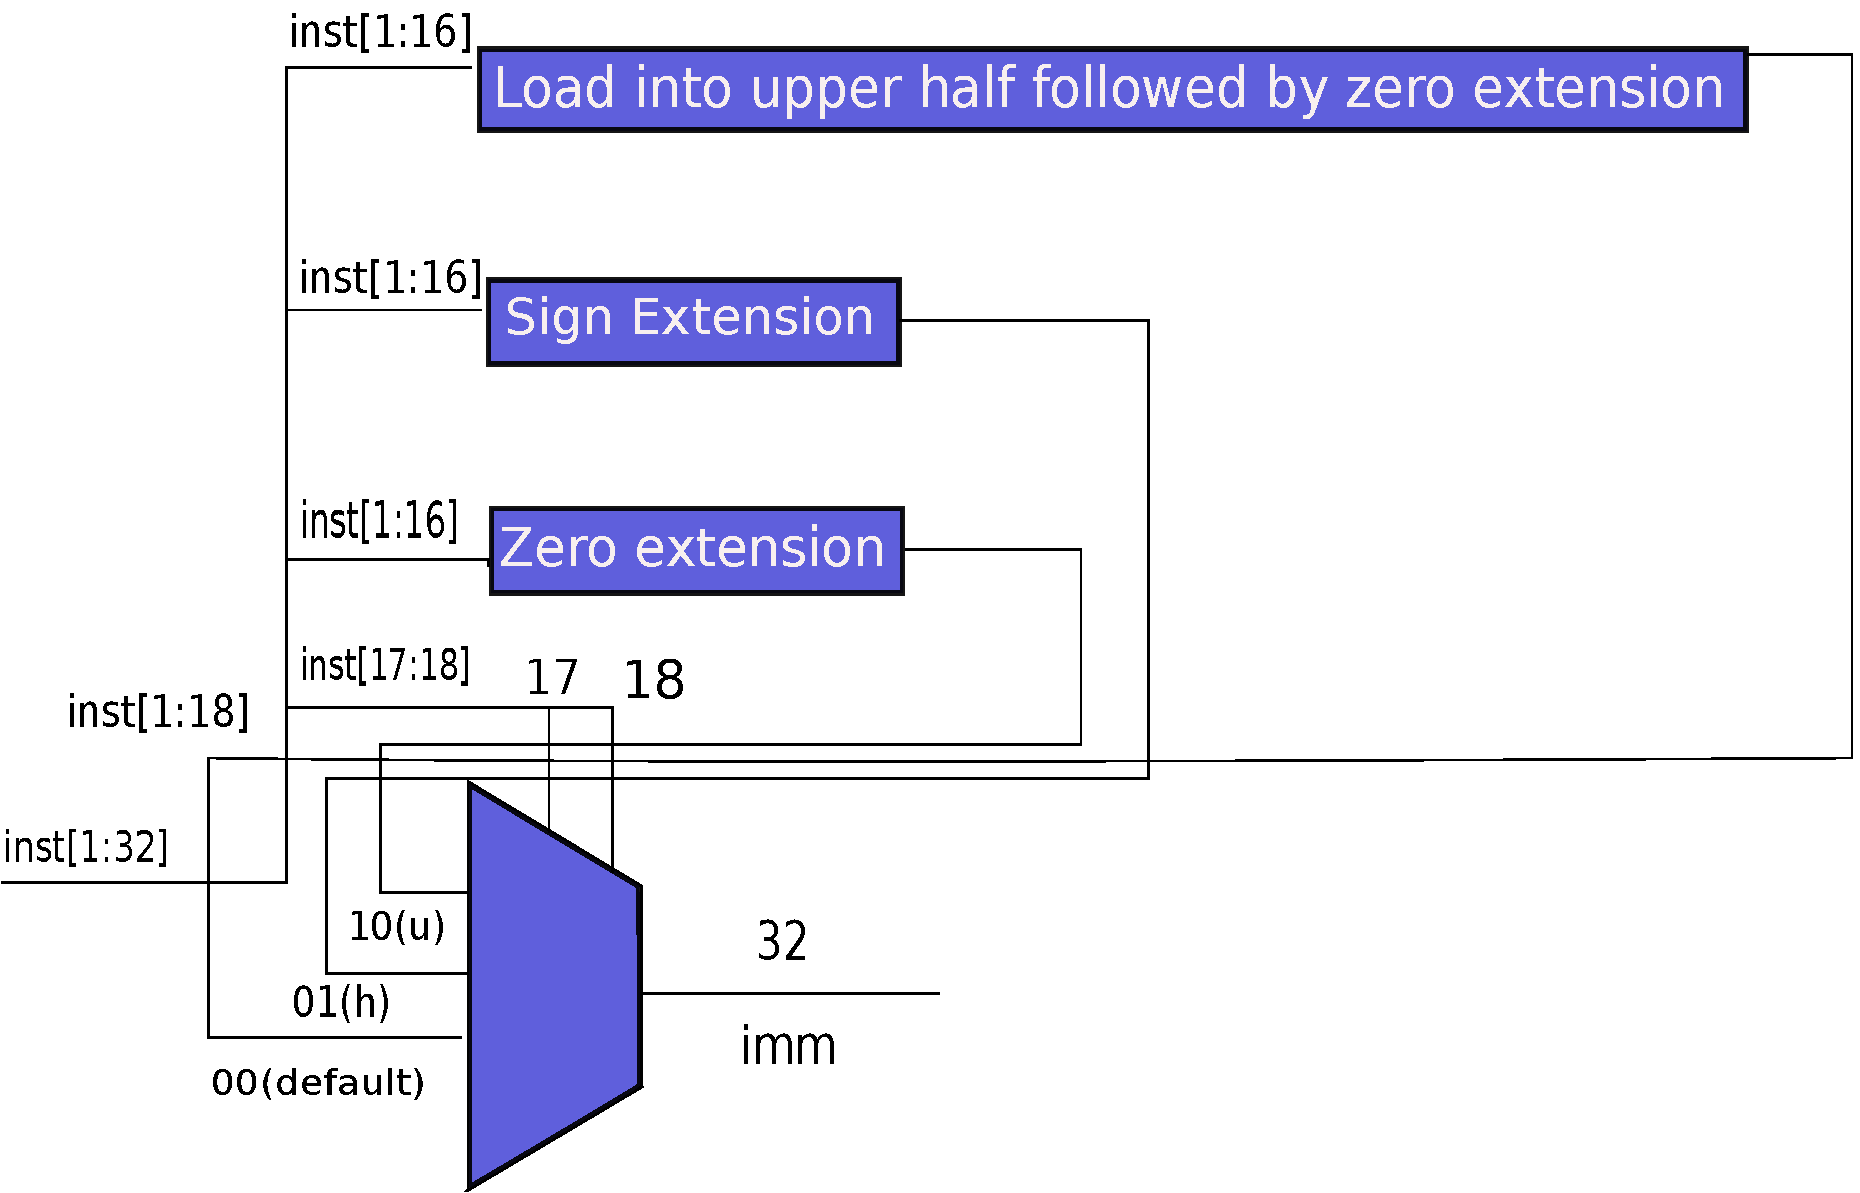
\includegraphics[width=10cm,height=8cm,keepaspectratio]{imm.pdf}
\end{figure}

\Exercise Why is it necessary for the register file in our \simplerisc processor
to have 2 read ports, and 1 write port?

\Answer
The \textit{SimpleRisc} instruction set has 21 instructions in its ISA. Looking at the list of instruction opcodes, it is clear that each instruction has atmost 2 read registers, and atmost 1 write back register. Hence, in the Instruction decode stage, it is necessary to have a Register file with 2 read ports and 1 write port for correct decoding.

\Exercise Why do we need 2 multiplexers in the OF stage of the processor? What are their
functions?

\Answer
The register file used in the decode(Operand Fetch) stage has 2 read ports and 1 write port. For the first register operand op1, we have two choices. For ALU,Memory instructions, we need to read the first source register,rs1. For \textit{ret},we need to read the value of the return register,\textit{ra}. In order to make a choice between the contents of the instruction fields \textit{rs1} or \textit{ra},we need to use a multiplexer. This is controlled by the control signal \textit{IsRet}. The output of the multiplexer is the input to the Register file's first read port, and is known as \textit{op1}.\newline
For instructions other than \textit{store}, the second source register is specified by \textit{rs2}. However, for the store instruction, we need to use the source register \textit{rd}. This choice between \textit{rs2} and \textit{rd} is made by using a second multiplexer. This is in turn, controlled by the \textit{isStore} signal. The output of the multiplexer is the input to the Register file's second read port and is known as \textit{op2}. \newline

\Exercise
Let us propose to compute the branch outcome and target in the OF stage. Describe the
design of the OF stage with this functionality.

\Answer
The operand fetch unit has two functions :1)calculate the values of the immediate operand and branch target 2)read the source registers\newline
The value of the immediate operand is calculated by extracting the \textit{imm} field from the instruction. The 32 bit value is calculated by extending the 18 bit \textit{imm} in accordance with the modifiers.\newline
The \textit{branchTarget} is calculated by first extracting the 27 bit offset, shifting by 2 bits and extending the sign. This is added to the PC to get the      \textit{branchTarget}.\newline
In case of the \textit{ret} instruction, the \textit{branchTarget} is the contents of the \textit{ra} register, read from the Register File. To choose between these two, a multiplexer is used, whose outcome is the required \textit{branchPC} value.\newline
The next part of the Fetch Unit is used to read the source registers and obtain the values of \textit{op1} and \textit{op2}. This is done with the help of the Register files, and the multiplexers.

\begin{figure}[H]
  \centering
  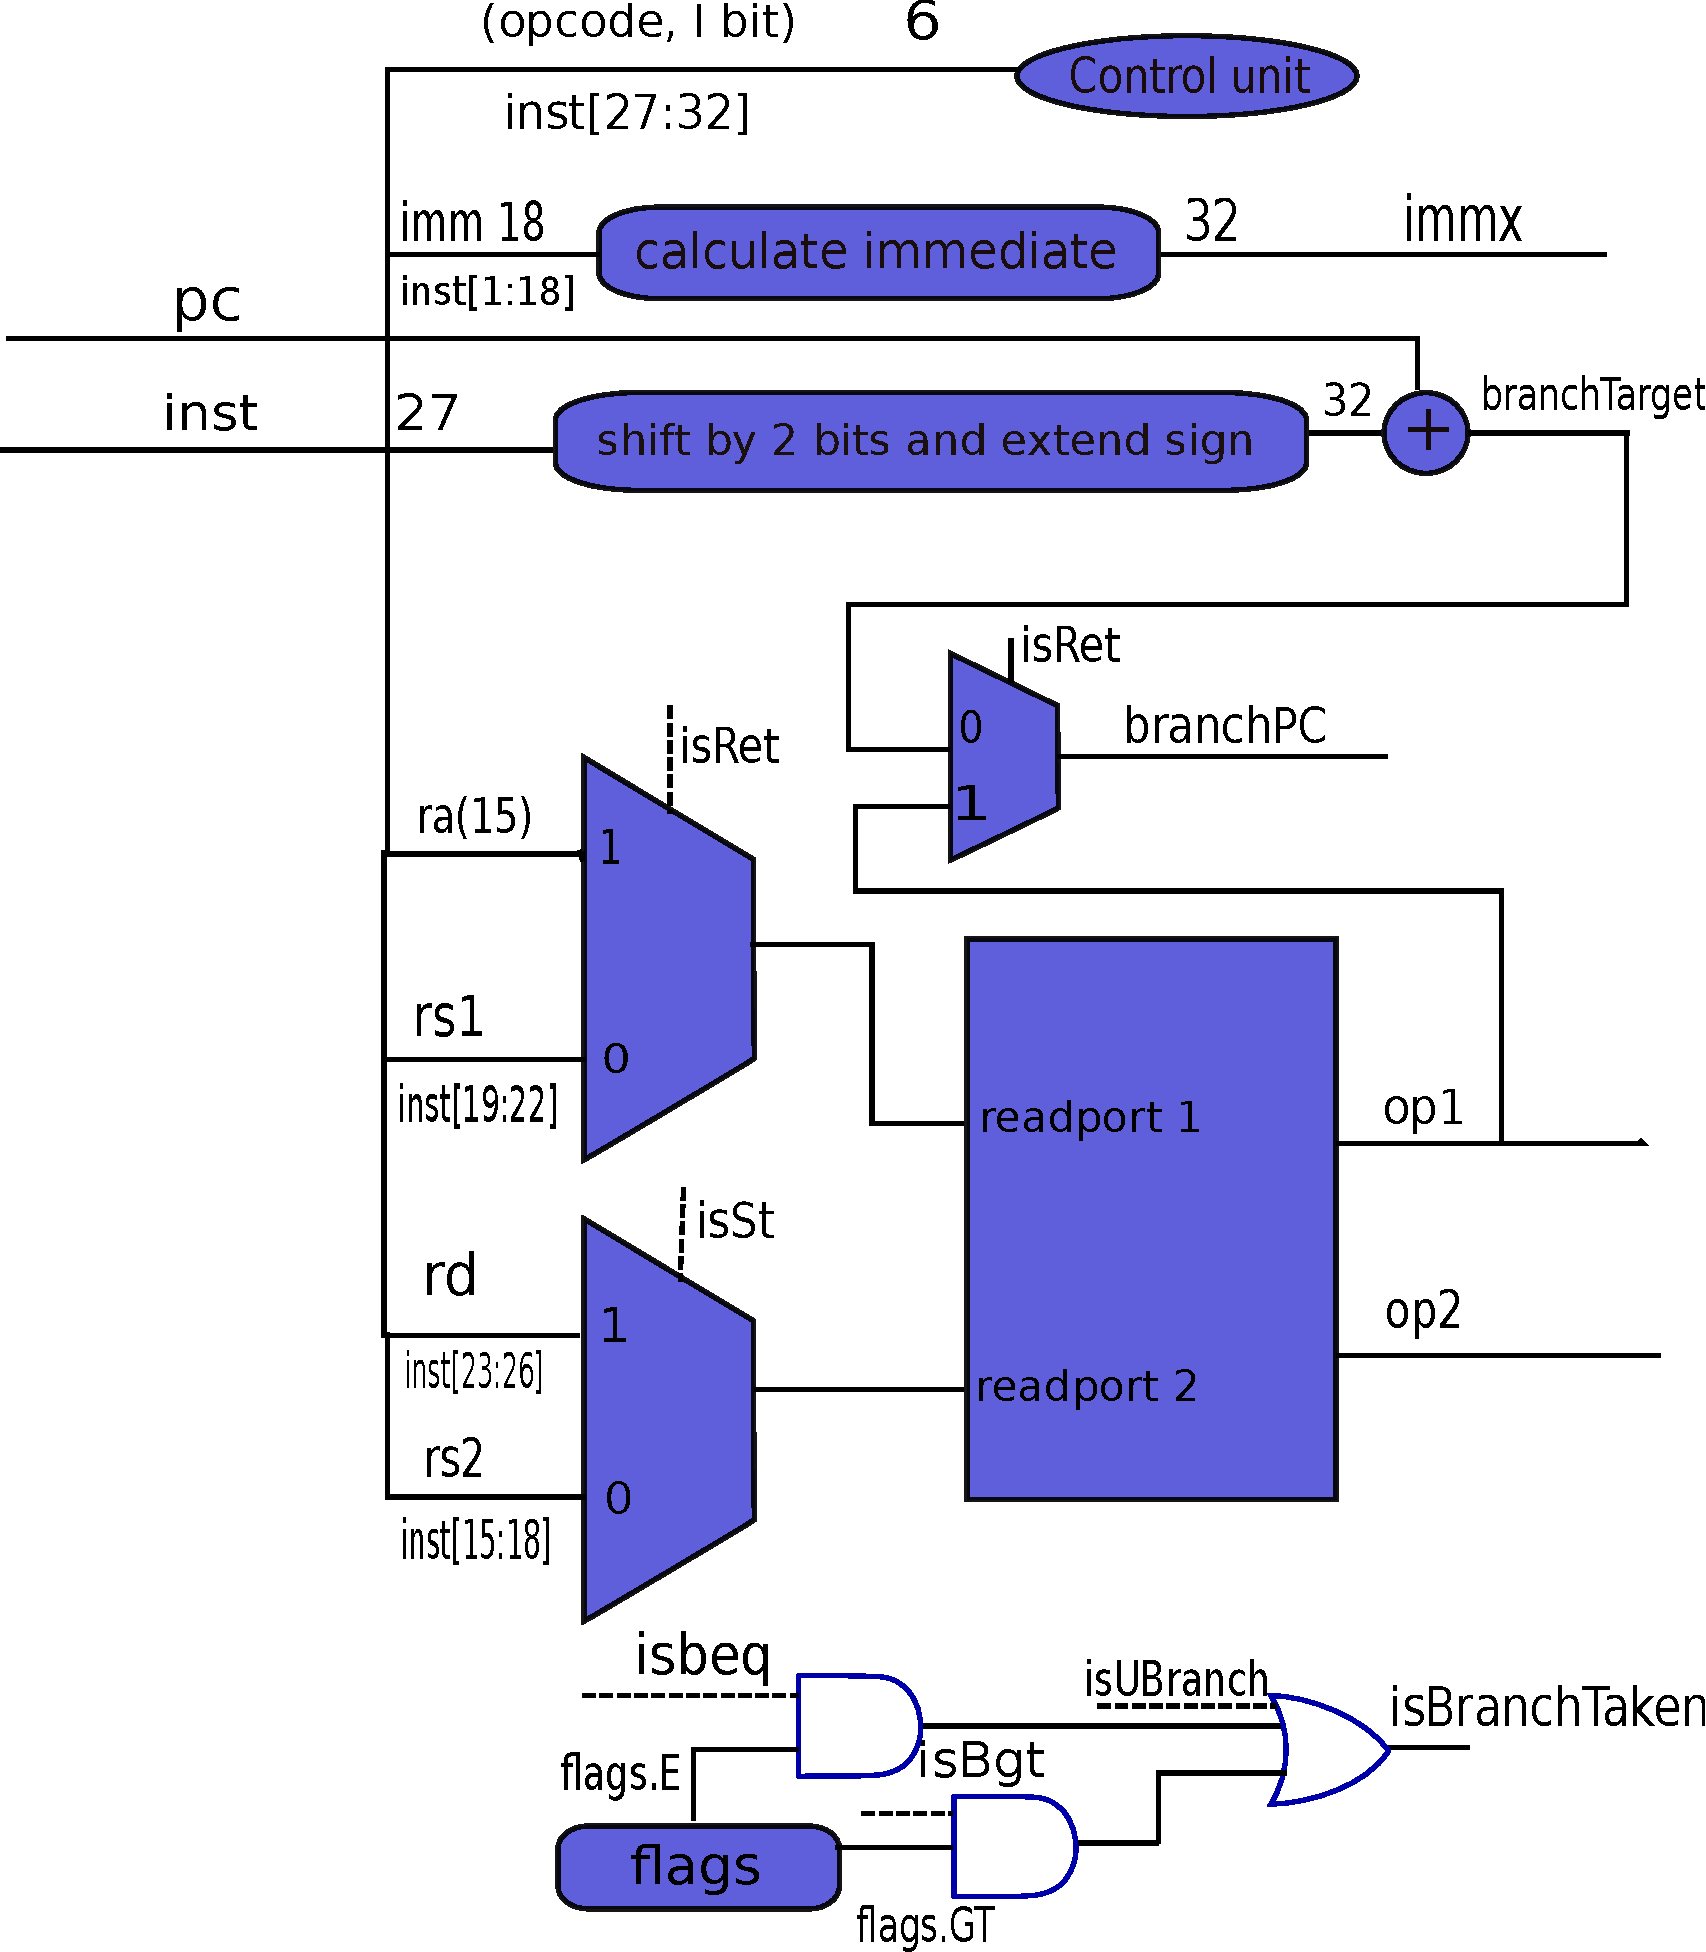
\includegraphics[width=10cm,height=10cm,keepaspectratio]{branch.pdf}
\end{figure}

\Exercise[difficulty=1]
For the ALU we use a multiplexer with a large number of inputs.
How can we implement this multiplexer
with transmission gates? (show a circuit diagram, and explain why your idea will
work) 
\Answer
\hspace{1mm} \\
The multiplexer can be implemented using tranmission gates. We use three select lines $S0$,$S1$,$S2$ to choose one of the outputs of the different modules of the ALU.
\begin{figure}[H]
  \centering
  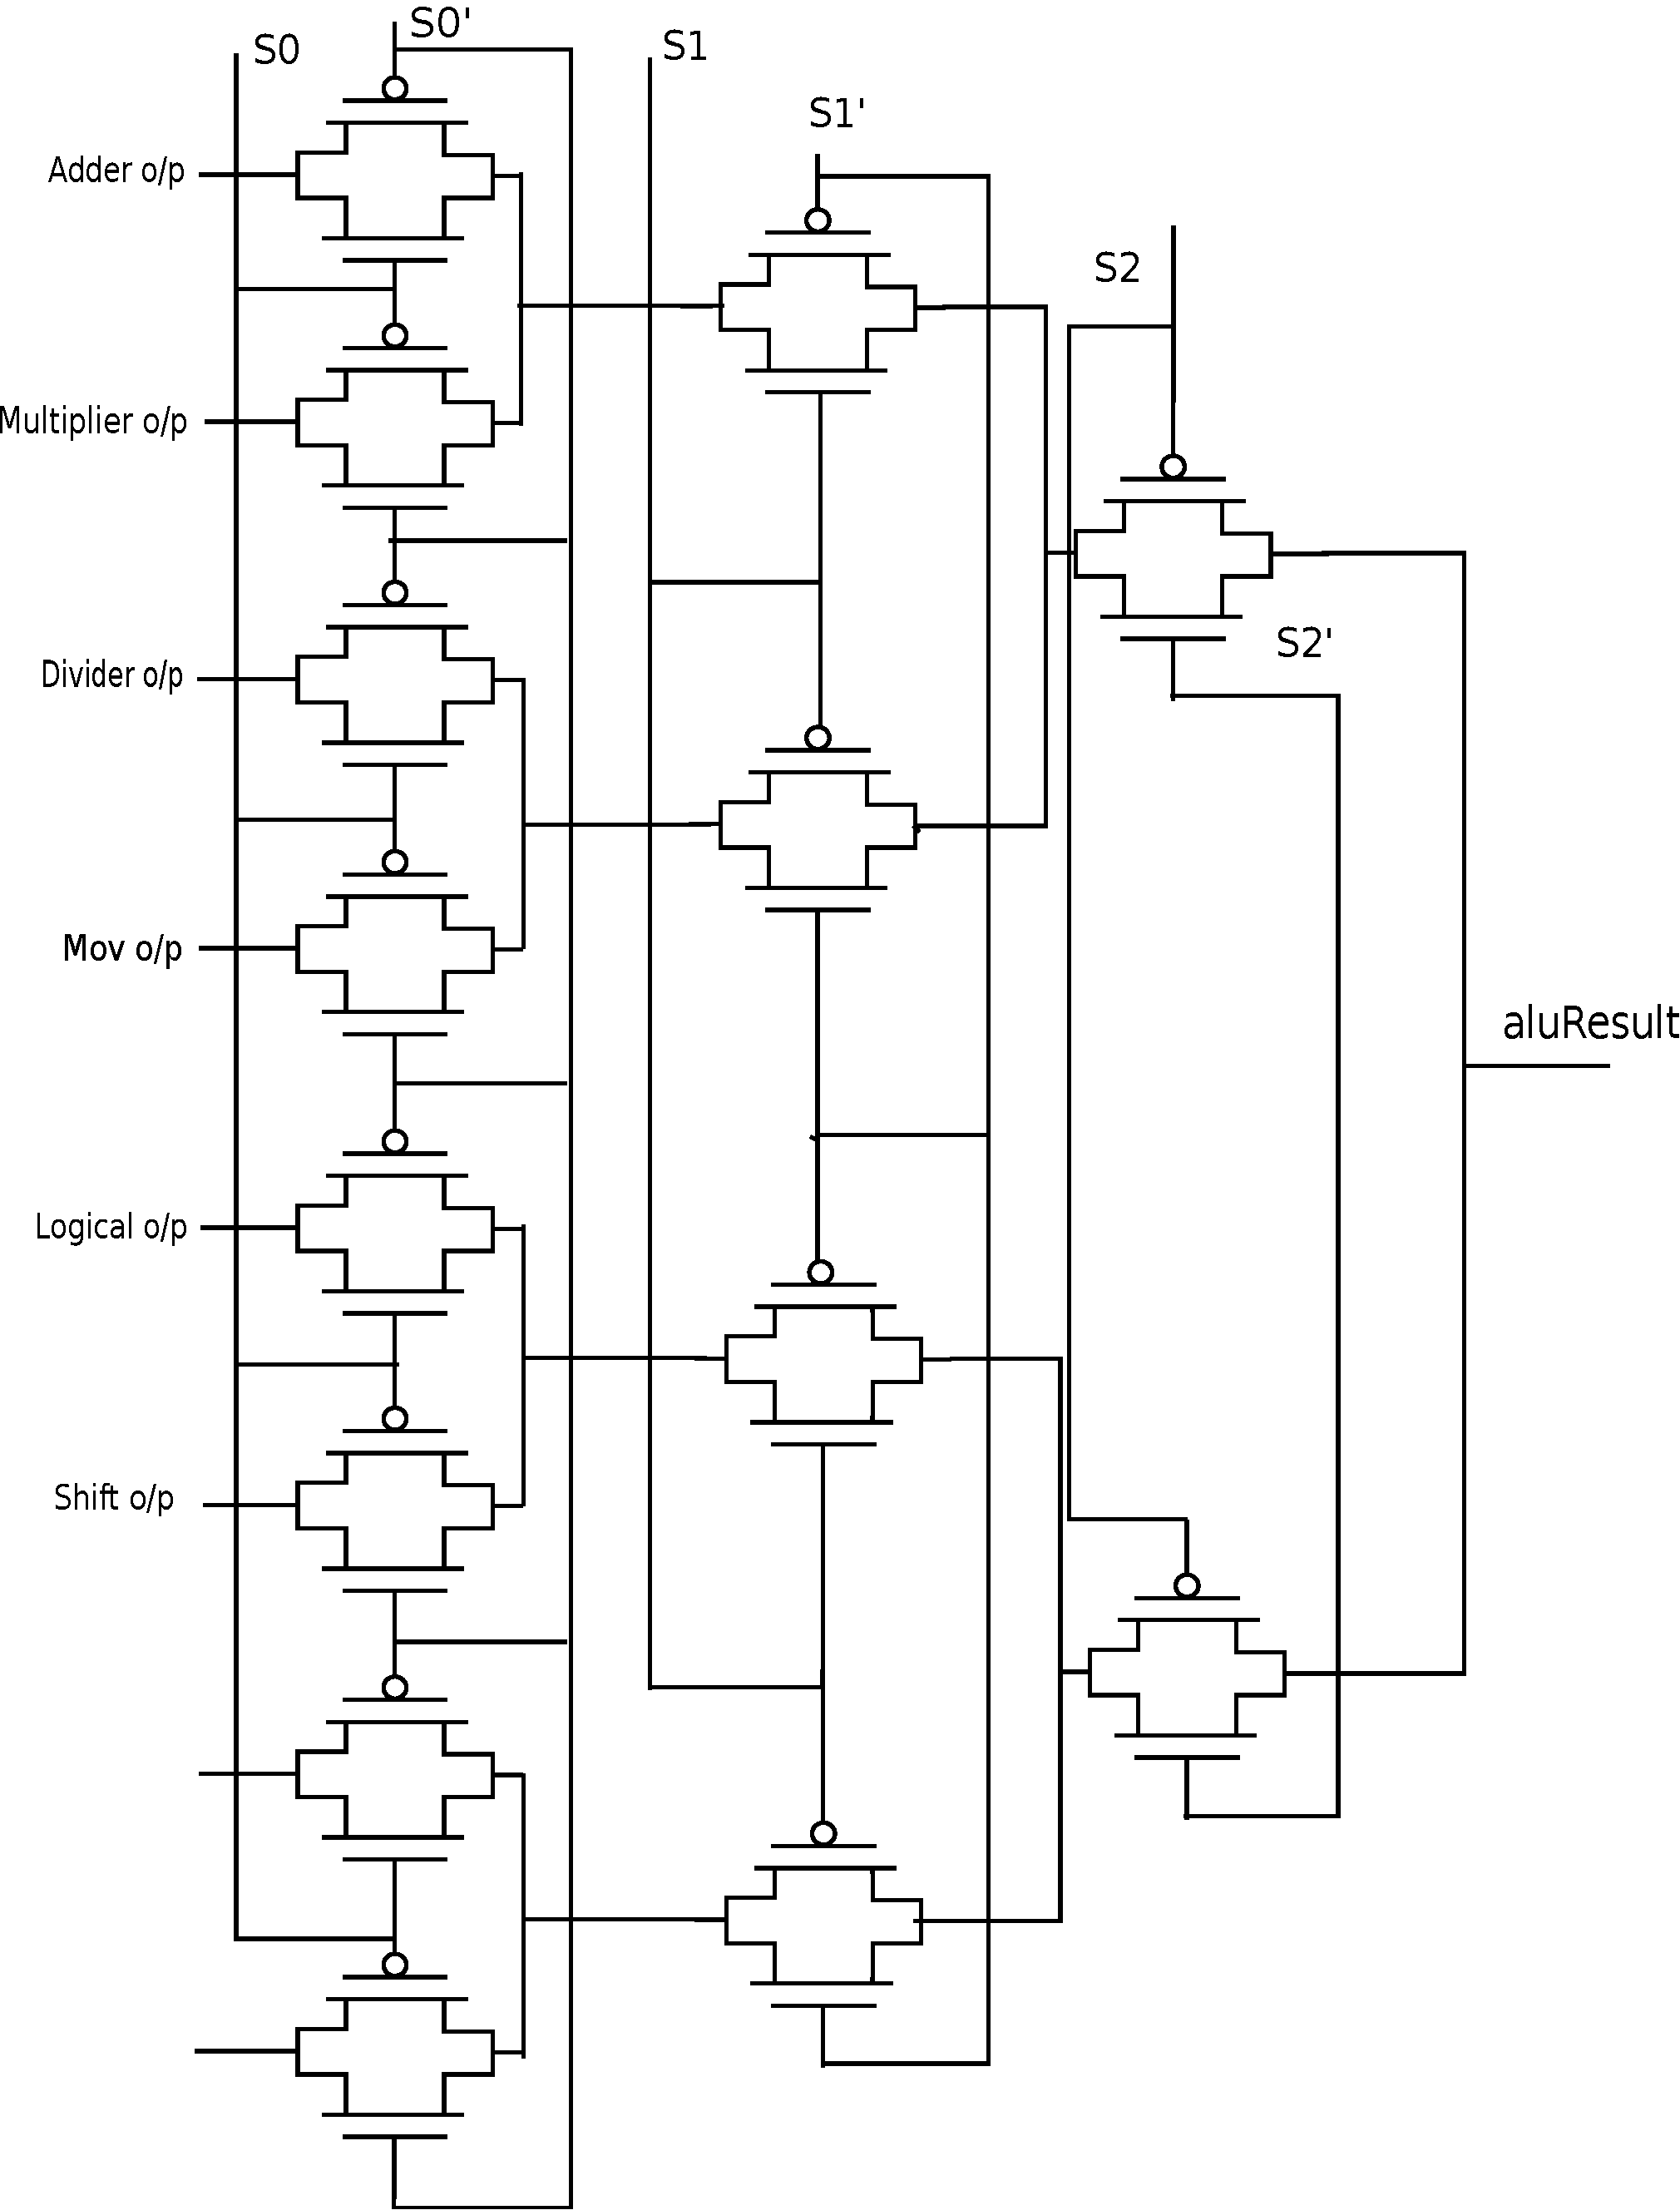
\includegraphics[width=10cm,height=14cm,keepaspectratio]{alu.pdf}
\end{figure}
\Exercise
Draw a circuit for implementing the $cmp$ instruction. It should show the subtraction, and the logic
for updating the flags.
\begin{figure}[H]
  \centering
  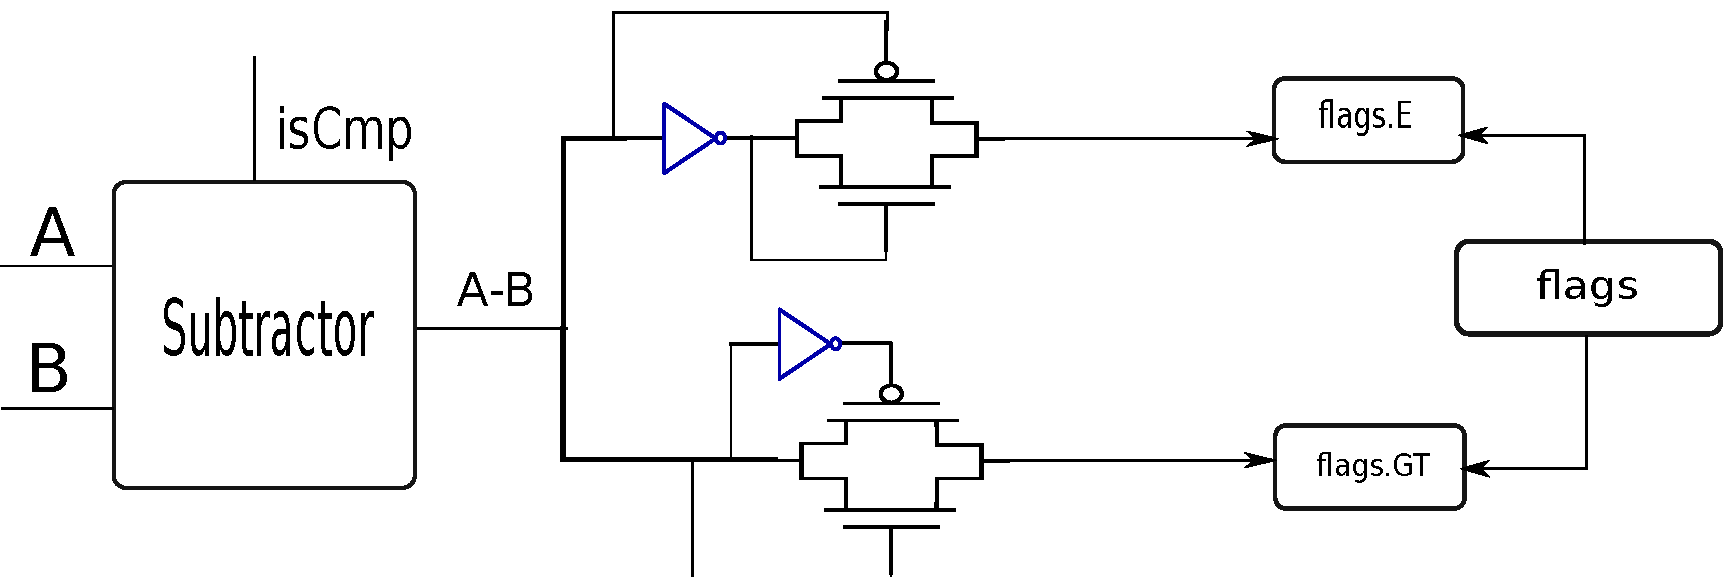
\includegraphics[width=10cm,height=7cm,keepaspectratio]{cmp.pdf}
\end{figure}
\Exercise
How do we implement the $call$ instruction in our processor?
\Answer
The call instruction is 1-address instruction as it takes only one argument-the label of the first instruction of the function. It transfers the control to the label and saves the return address in register \textit{ra}.
For the call instruction, the \textit{isBranchTaken} signal is turned on, and using the value of the \textit{branchPC} from the decode unit, the value of \textit{pc} register is updated.
The \textit{branchTarget} value is calculated using the 27 bit offset in instruction. This is shifted by 2 bits to get a 29 bit number which is then sign extended to obtain a 32 bit offset. This is added to the value in the \textit{pc} register to obtain the address of the function.
The return address is equal to the PC of the \textit{call} instruction plus 4. In the Register Writeback unit, we use a multiplexer to choose between the  \textit{aluResult}, \textit{ldResult},PC plus 4. For the \textit{call} instruction,
the \textit{isCall} is equal to 1, and hence we choose PC + 4. This is written back to the register file.

\Exercise
Show the circuit diagram for computing the $isWb$ signal.
\begin{figure}[H]
  \centering
  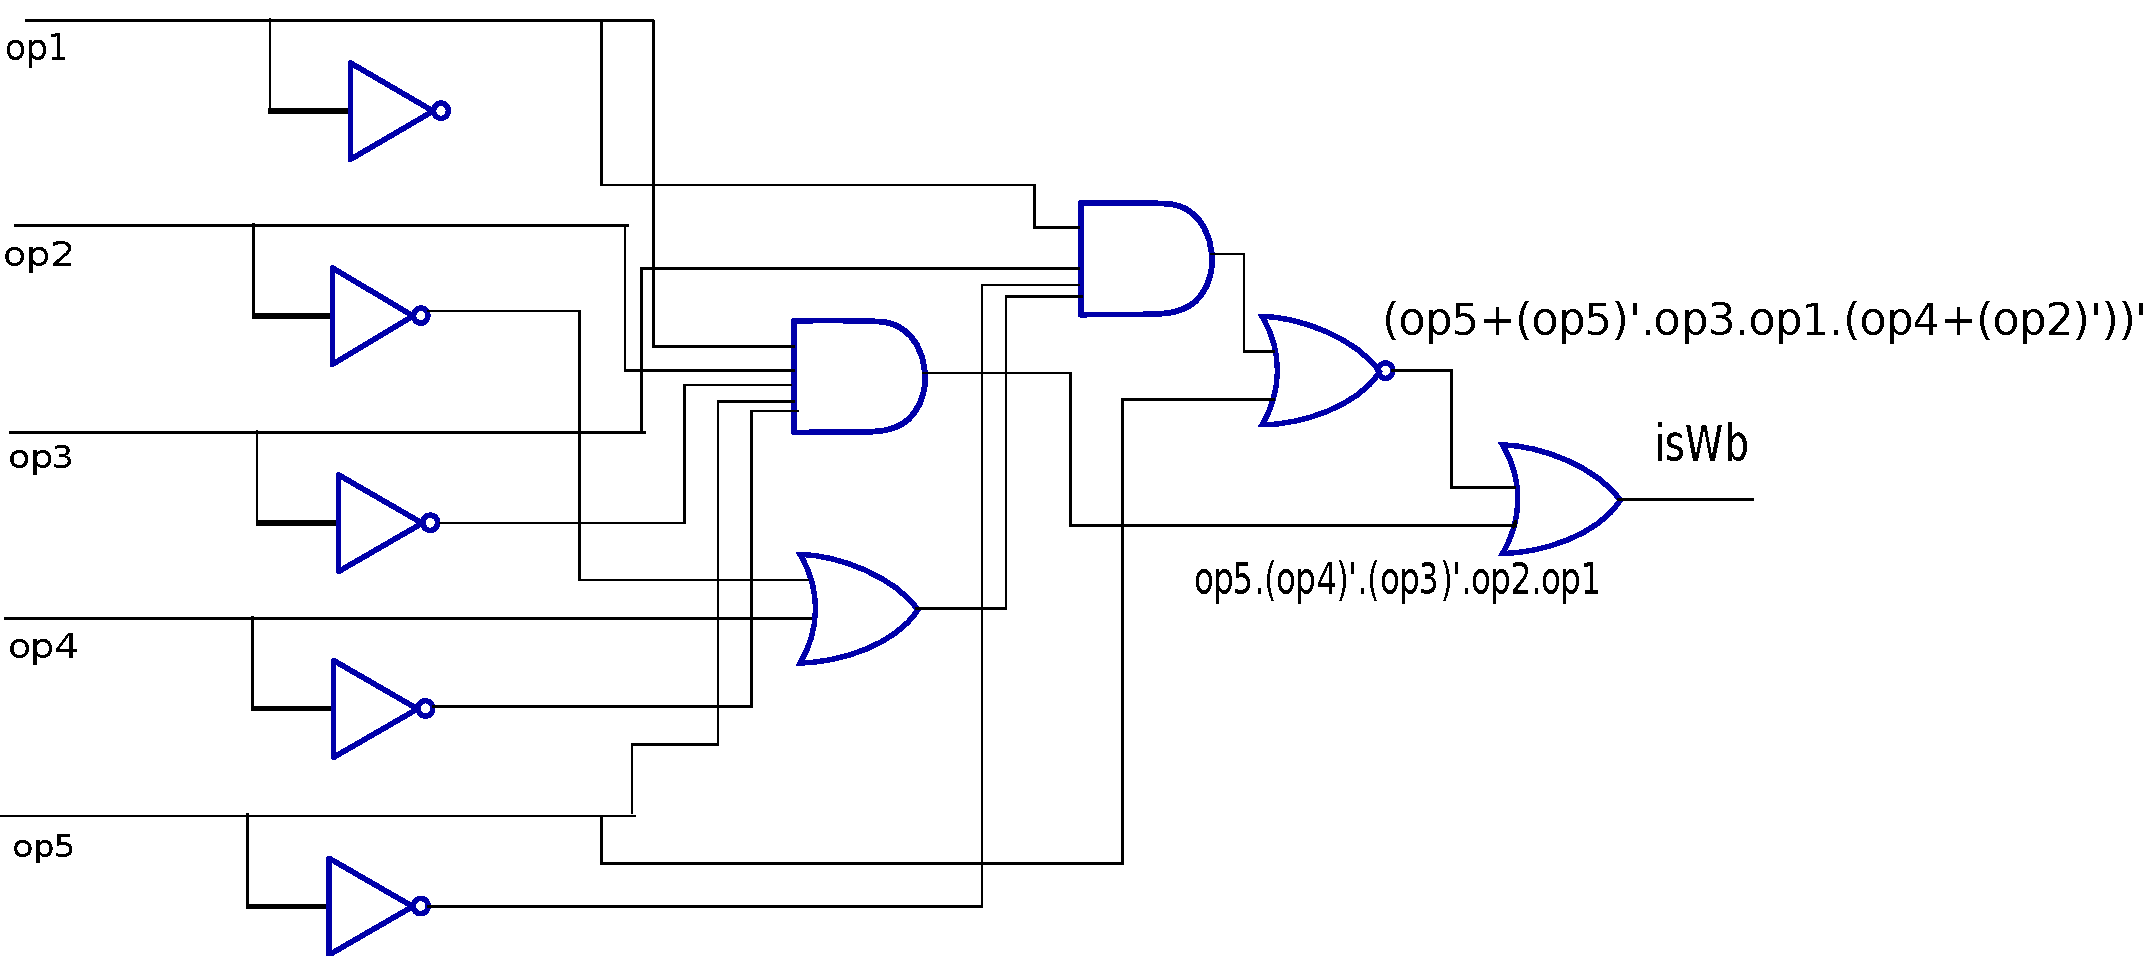
\includegraphics[width=10cm,height=7cm,keepaspectratio]{isWb.pdf}
\end{figure}
\Exercise
Why do we use the $isAdd$ control signal for the load, and store instructions also?

\Answer
The \textit{ld} and \textit{st} instructions use the values - \textit{rd,rs1} and \textit{imm}. The load instruction computes the memory address by computing the sum of contents of \textit{rs1} and \textit{imm}, which is done by the adder of the ALU in the execute stage. It then accesses the memory address and loads its contents to the \textit{rd} register.
The store instruction stores the value of \textit{rd} into the memory address given by contents of \textit{rs1} + \textit{imm}. To compute this, it uses the adder of the ALU in the execute stage.
Hence, for both these instructions, we use \textit{isAdd} control signal to enable the adder of the ALU.
\end{ExerciseList}

\section*{Microprogramming}

\begin{ExerciseList}

\Exercise Compare a hardwired control unit and a microprogrammed control unit.
\Answer
A hardwired processor has a datapath with all the elements required to process and execute an instruction. To incorporate the choice between two input operands, a multiplexer , controlled by a signal from the control unit is added. The control unit takes the instruction contents , and generates all the control signals. 

A microprogrammed processor uses a translation table that translates instructions in the ISA to a set of simple microinstructions. Each microinstruction has access to all the latches, and internal state elements of a processor. The functionality of an instruction is realised by the execution of the set of microinstructions associated with it. These are called \textit{microcodes} and are stored in a microcode table, which can be modified.

Hardwired processors are high performance processors and are used for devices where speed is crucial. However, this comes with a cost on flexibility. Introduction of new instructions or modifying the method of execution of an existing instruction is not possible once designed and shipped.

On the other hand, microprogrammed processors are flexible as the contents of the microcode table can be modified. This flexibility allows addition of new instructions or alteration of method of execution of existing ones. However, the speed is reduced in comparison to the hardwired processors. 
\Exercise Draw the block diagram of a microprogrammed processor.

\begin{figure}[H]
  \centering
  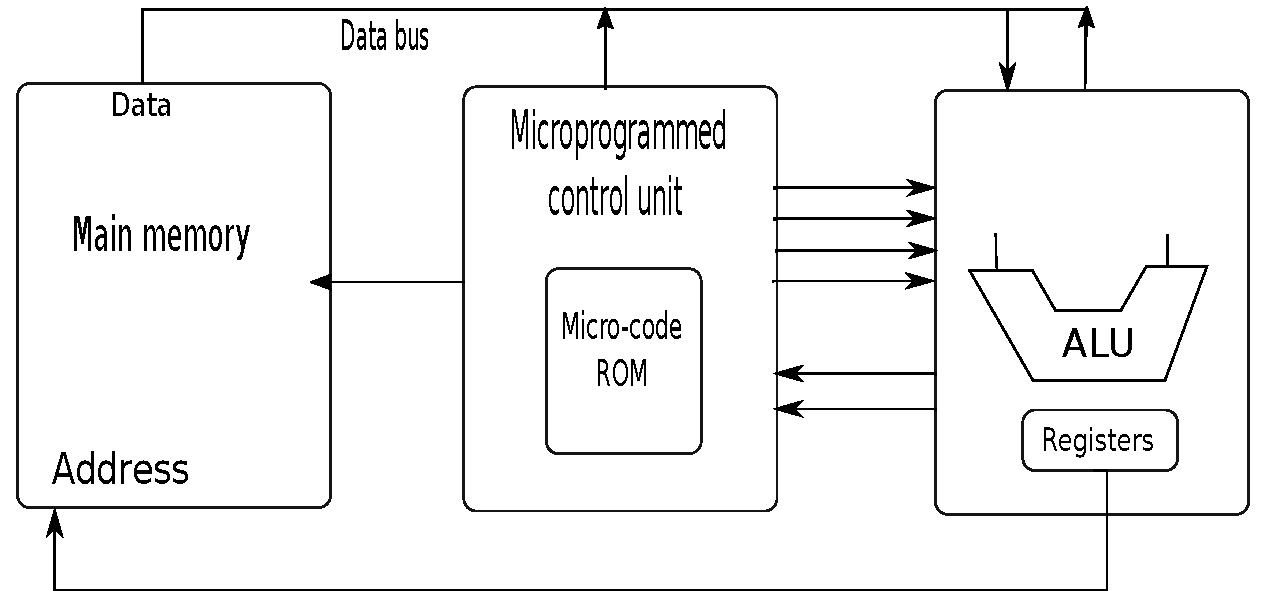
\includegraphics[width=10cm,height=7cm,keepaspectratio]{mcu.pdf}
  \caption{Block diagram of microprogrammed processor}
\end{figure}

\Exercise Why do we need the $mswitch$ instruction.
\Answer
The microprogrammed processor has a set of microinstructions associated with every instruction. These are stored in the microcode table. Once the contents of the instruction are loaded into the \textit{ir} register using \textit{mloadIR} microinstruction, and is decoded using \textit{mdecode}, we need to load the microinstructions corresponding to the instruction being referred to. This is accomplished by using the \textit{mswitch} instruction.
It makes the $\mu$ control unit to jump to the appropriate location in the microinstruction memory, and starts executing microinstructions starting from that location. 
\Exercise
Show the microcode implementation of the load and store instructions.
\Answer :

.begin\newline
mloadIR\newline
mdecode\newline
add pc,4\newline
mswitch\newline
\newline
ld instruction :\newline

/* transfer rs1 to register A*/\newline
mmov regSrc,rs1, $\langle$ read $\rangle$ \\
mmov A,regVal\newline
\newline
/* calculate the effective address */\newline
mmov B,immx, $\langle$ add $\rangle$ /* ALU operation */ \\
\\
/* perform the load */\newline
mmov mar,aluResult, $\langle$ load $\rangle$ \\
\newline
/*write the loaded value to the register file */\\
mmov regData,ldResult\newline
mmov regSrc,rd, $\langle$ write $\rangle$ \\
\newline
/* jump to the beginning */\newline
mb .begin \newline
\newline

The value of the first source register is transferred to the ALU. Then,the value of the immediate is transferred to the second ALU register(B), and the add operation to calculate the effective address is initiated. Once the effective address is calculated, it is available in \textit{aluRegister}. The contents of the \textit{aluRegister} are moved to the memory address register \textit{mar}, and the load operation is initiated. The result is available in the \textit{ld} register in the next cycle. This is then written to the register specified by \textit{rd} in the next two cycles.\newline
\newline
st instruction :
\newline

/* transfer rs1 to register A*/\newline
mmov regSrc,rs1, $\langle$ read $\rangle$ \newline
mmov A,regVal\newline
\newline
/* calculate the effective address */\newline
mmov B,immx, $\langle$ add $\rangle$ /* ALU operation */\newline
\newline
/* perform the store */\newline
mmov mar,aluResult\newline
mmov regSrc,rd, $\langle$ read $\rangle$\newline
mmov mdr,regVal,$\langle$ store $\rangle$\newline
\newline
/* jump to the beginning */\newline
mb .begin \newline \\
The store function works in a similar way. The effective memory address is first calculated and stored in the \textit{mar} register. Then, the value of the \textit{rd} register that contains the data to be stored is read. This, in turn, is saved to the \textit{mdr} register, and the store operation is issued.
\Exercise
Write a program in microassembly to check if a number in register $r2$ is a perfect square. Save the Boolean result
in register, r0.
\Answer :

.begin\newline
mloadIR\newline
mdecode\newline
add pc,4\newline
mswitch\newline \\
mmovi B,1   /*stores the odd number being added*/\newline
mmovi regSrc,2,$\langle$ read $\rangle$\newline
mmov A,regVal\newline \\
/*loop*/\newline
.loop:\newline
/*Compute subtraction*/\newline
mmov A,A,$\langle$ sub $\rangle$\newline
mmov A,aluResult\newline
madd B,1    /*B=B+1*/\newline
madd B,1    /*B=B+1*/\newline
mbeq A,0,.success   /*n =1+3+5+7.. , hence is a perfect square, branch to .success*/\newline
mmov sr1,A\newline
mmov sr2,B\newline
mmovi A,0   /*A=0*/\newline
mmov B,sr2,$\langle$ cmp $\rangle$\hspace{3mm}/*B=sum of odd numbers*/\newline
mbeq flags.GT,1,.failure  /*If the sum of odd numbers exceeds n, then n is not a perfect square, branch to .failure*/\newline
mmov A,sr1\newline
mmov B,sr2\newline
mb .loop\newline
\newline
.success:\newline
mmovi regSrc,3\newline
mmovi regData,1,$\langle$ write $\rangle$\newline
mb .begin\newline
\newline
.failure:\newline
mmovi regSrc,3\newline
mmovi regData,0,$\langle$ write $\rangle$\newline
mb .begin\newline \\ \\

The program uses the logic that a perfect square can be expressed as a sum of odd numbers 1+3+5+7+9... .Thus, from the original number, we keep subtracting every odd number beginning from 1. If we end up with a zero, then the given number is a perfect square. However, if it turns out to be a negative number, then it isn't. Hence, we break out of the loop in either case and branch to different functions.\newline
Assumption: sr1 and sr2 are scratch registers

\Exercise
Write a program in microassembly to check if the value in register $r2$ is a palindrome. A palindrome
reads the same from both sides. For example, the 8 bit number, 11011011 is a palindrome. Save the Boolean result
in register, r0.
\Answer:

.begin\newline
mloadIR\newline
mdecode\newline
add pc,4\newline
mswitch\newline \\
mmovi B,0  /*Loading count into B*/\newline
mmovi regSrc,2,$\langle$ read $\rangle$\newline
mmov A,regVal\newline \\ 
mmov sr2,B  /*sr2 holds the value of count*/\newline
mmov sr1,A  /*sr1 holds the value of original number*/\newline
mmovi A,1   /*To perform 1 $\ll$ count*/ \\
.loop:\newline
mbeq sr2,16,.success /*breaking out of loop if count==16*/\newline
mmov B,B,$\langle$ lsl $\rangle$  /*aluResult=1 $\ll$ count*/\newline
mmov sr2,B  /*sr2 holds count*/\newline
mmov A,aluResult  /*A=aluResult*/\newline
mmov B,sr1,$\langle$ and $\rangle$    /*x=num and (1 $\ll$ count)*/\newline
mmov sr3,aluResult  /*sr3 holds lsb*/\newline \\
mmovi A,31\newline
mmov B,sr2,$\langle$ sub $\rangle$   /*aluResult=31-count*/\newline
mmov B,aluResult\newline
mmov A,sr1,$\langle lsr \rangle$  /*aluResult=(num $\ll$ (31-count))*/\newline
mmov A,aluResult\newline
mmovi B,1,$\langle and \rangle$ \hspace{3mm}/*y=(num $\gg$ (31-count)) $\and$ 1*/\newline \\
madd sr2,1 /*count=count+1*/\newline
mmovi A,1  /*A=1*/\newline
mmovi B,sr2  /*B=count*/\newline
mbeq sr3,aluResult,.loop  /*Loop if x==y */\newline
/*x and y are count th bits from left and right*/\newline
.failure\newline
mmovi regSrc,3\newline
mmovi regData,0,$\langle write \rangle$ \newline
mb .begin\newline
.success\newline
mmovi regSrc,3\newline
mmovi regData,1, $\langle write \rangle$ \newline
mb .begin\newline    
\newline
Assumption: sr1,sr2 and sr3 are scratch registers
\Exercise[difficulty=1]
Write a program in microassembly to check if the value in register $r2$ can be expressed as a sum of two
cubes in two different ways. For example, 1729, is one such number. $1729 = 12^3 + 1^3 = 10^3 + 9^3$. Save the Boolean result
in register, r0.

\Exercise
Outline the design of the shared bus, and microprogrammed data path. Explain the functionalities of each of its
components.
\Answer
The shared bus consists of two buses - write bus and read bus.\newline
The first bus,\textit{write bus} is connected to all the registers that might write data into the bus. The output of the write bus,the embedded immediate($\mu$ imm) in the microinstruction, and the output of the $\mu$adder are sent to a multiplexer. The $\mu$adder adds the embedded immediate with the register contents. Now, this multiplexer chooses one value among the three, and sends it onto a read bus. This multiplexer is referred to as \textit{transfer multiplexer}. All the registers that might potentially read a value are connected to the read bus. The PC is connected to both the buses. The $\mu$adder has two inputs. One of them is the sign extended immediate that is a part of the microinstruction, and the other is the output of the write bus.\newline
The value sent on the write bus is compared with $\mu$imm . The result is contained in the \textit{isMBranch} signal. This is required for the implementation of \textit{mbeq} instruction.
\newline \textbf{Microprogrammed Datapath}\newline \\
1.\hspace{4mm}\textit{Fetch Unit}:\newline 
It consists of two registers-\textit{pc} and \textit{ir}, PC and instruction register respectively.\textit{ir} contains the contents of the instruction. The \textit{pc} register can read or write to the bus. The \textit{pc} is connected to the instruction memory and bus. \textit{ir} is connected only to the instruction memory.\newline \\
2.\hspace{4mm}\textit{Decode Unit}:\newline 
The decode unit breaks the instruction contents into multiple fields, and exports as registers-\textit{I,rd,rs1,rs2,immx,branchTarget}. The offset from the current PC is calculated by extracting [1:27] bits from the instruction register \textit{ir}, and shifting by two places. The offset thus calculated ,is added to the PC.\newline \\
3.\hspace{4mm}\textit{Register File}:\newline 
It has two source registers-\textit{regSrc} and \textit{regData}.The \textit{regSrc} register contains the number of the register to be accessed.In case of a write,the \textit{regData} register contains the value to be written. The \textit{args} values are directly read from the bus. They contain the commands to the register file-\textit{read,write,nop}.If \textit{args} specifies a \textit{write} operation,then the value in the \textit{regData} is written to the \textit{regSrc}.If its a \textit{read} operation, then the register specified by \textit{regSrc} is read and stored in \textit{regVal}.\newline \\
4.\hspace{4mm}\textit{ALU}:\newline 
The ALU consists of two registers, A and B.The ALU performs actions on the values contained in the registers,A and B. The nature of the operation is specified by the \textit{args} value. For all other instructions other than \textit{cmp}, the result is stored in the \textit{aluResult}, whereas for \textit{cmp}, it gets stored in either of the two registers-\textit{flags.E},\textit{flags.GT}.\newline \\
5.\hspace{4mm}\textit{Memory Unit}:\newline 
It has two source registers-\textit{mar,mdr}.The memory address register buffers the memory address, and memory data register buffers the value to be stored.If the operation specified by \textit{args} is a load, then the result is stored in \textit{ldResult}.\newline
 
\Exercise
Draw a detailed diagram of the $\mu$control unit along with the transfer multiplexer in a vertically microprogrammed
processor.
\begin{figure}[H]
  \centering
  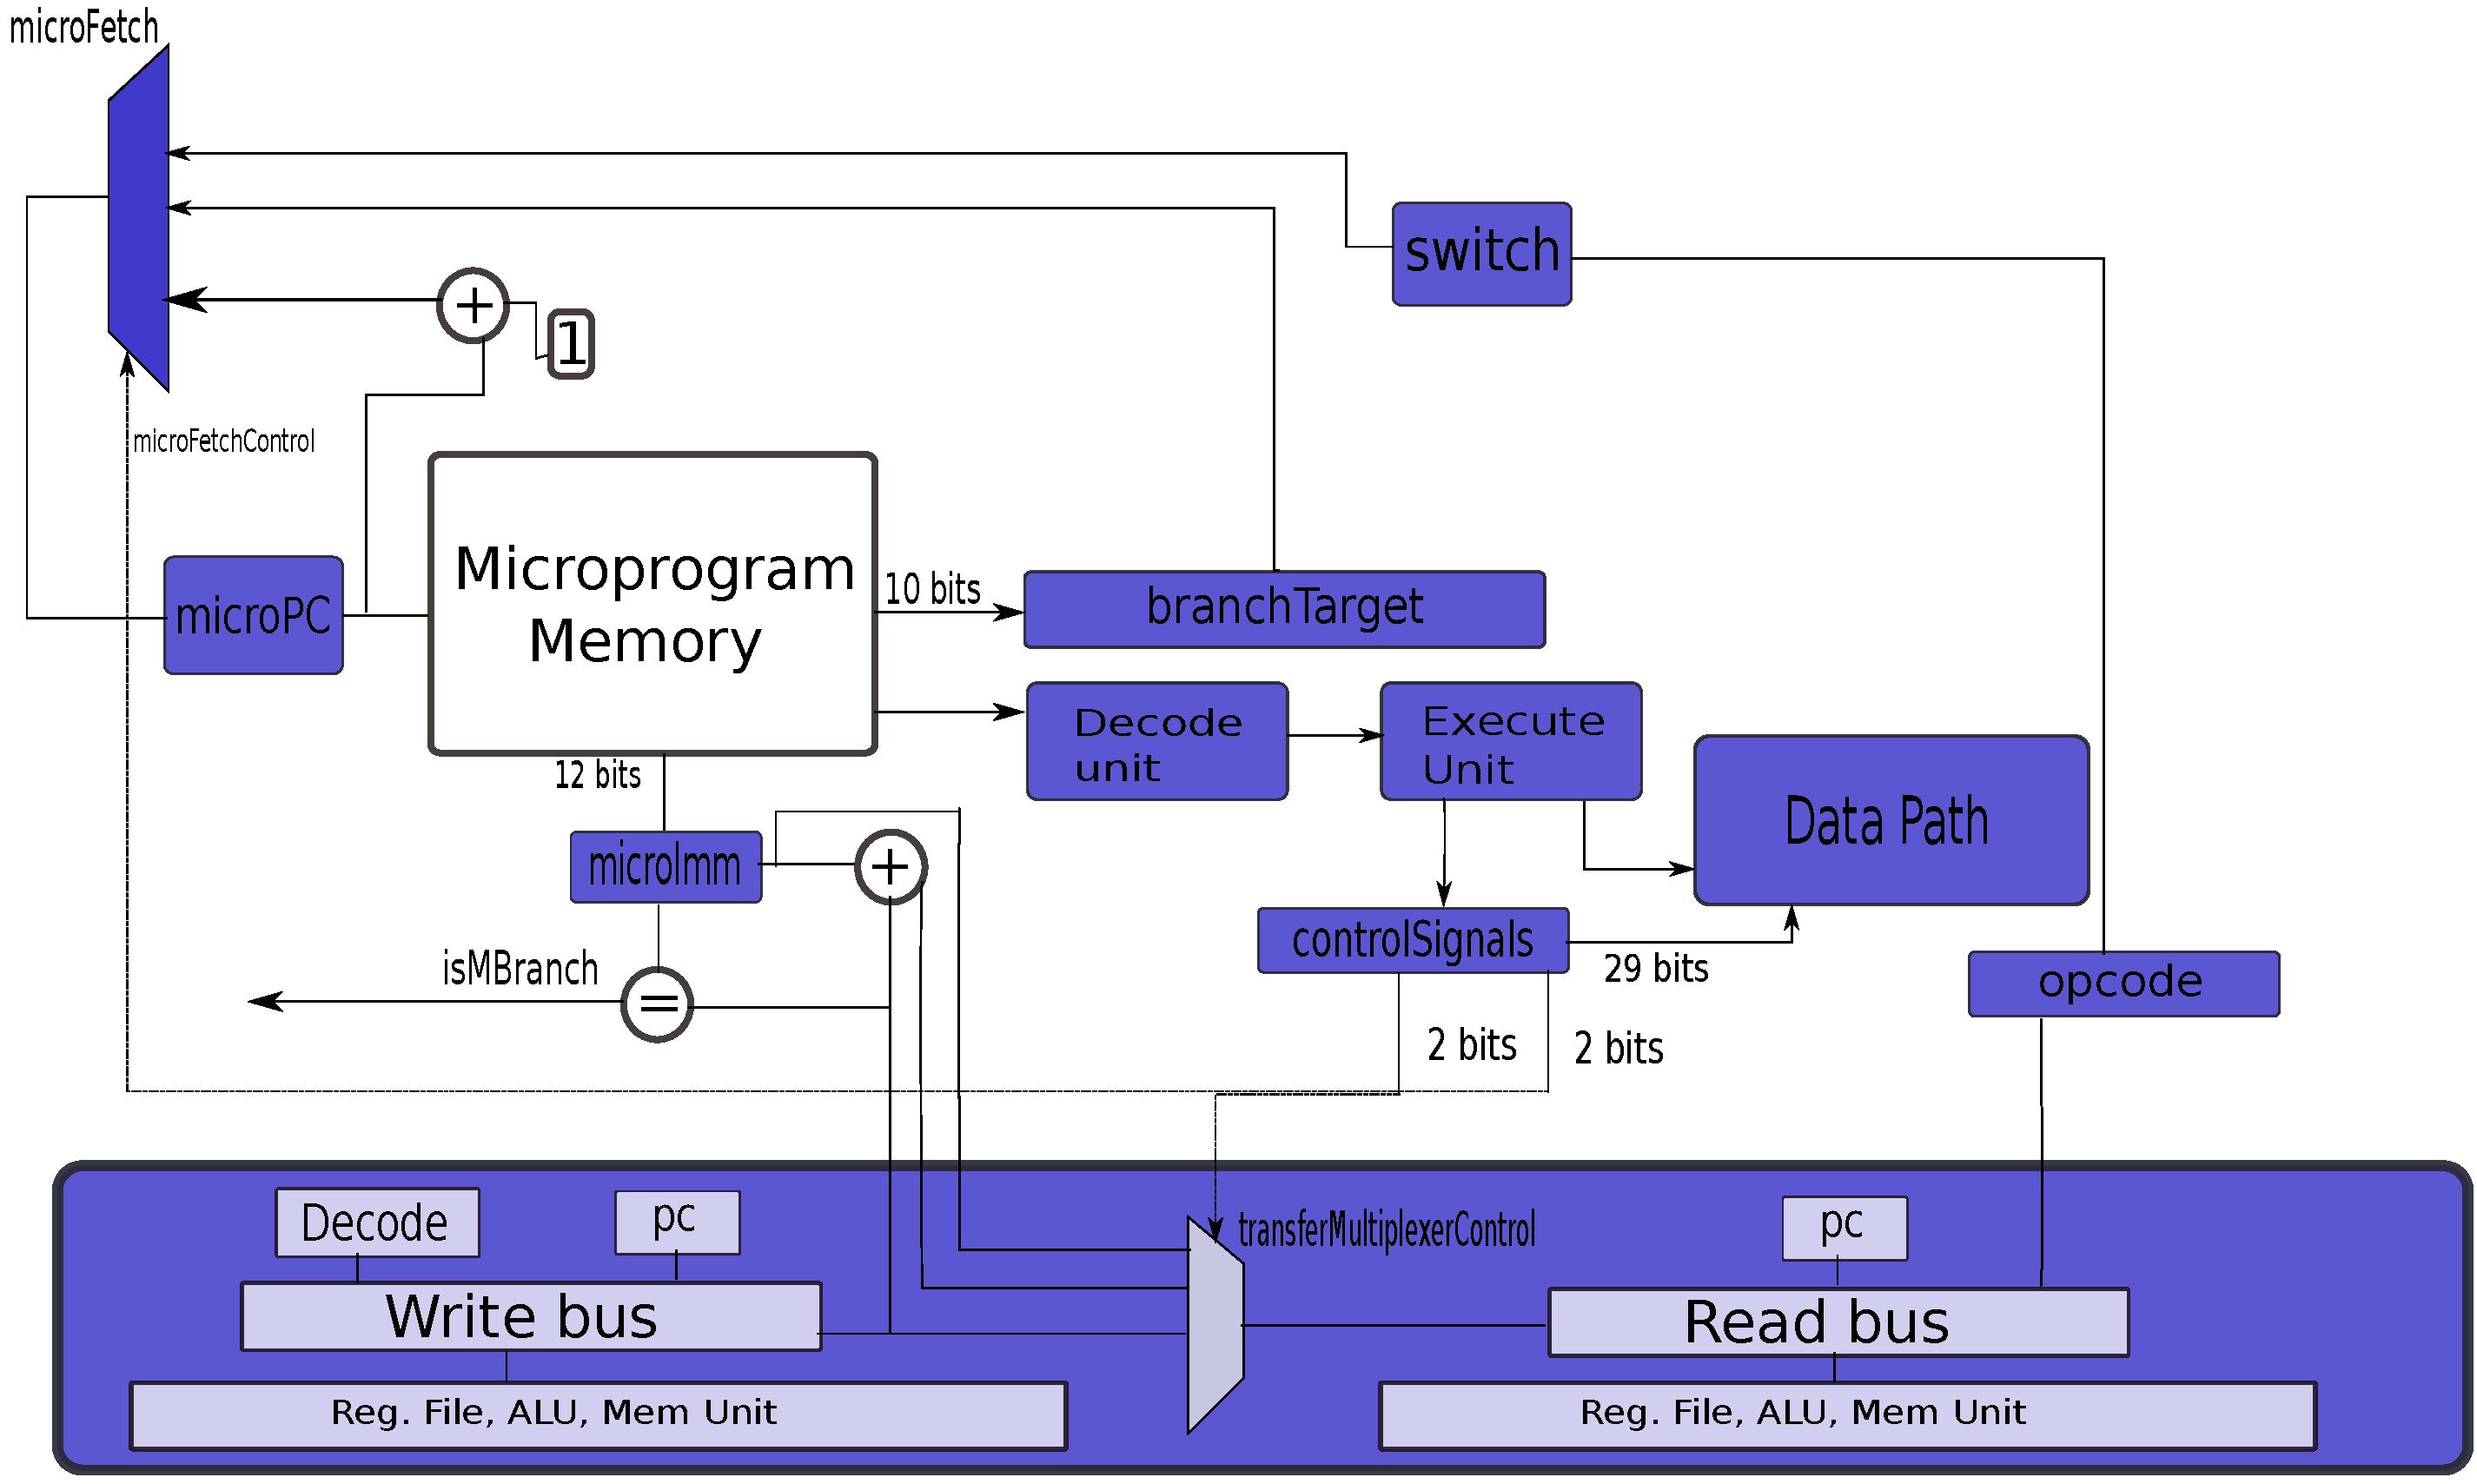
\includegraphics[width=12cm,height=14cm,keepaspectratio]{verticalMP.pdf}
\end{figure}
\Exercise
Draw a detailed diagram of the $\mu$control unit along with the transfer multiplexer in a horizontally microprogrammed
processor.
\begin{figure}[H]
  \centering
  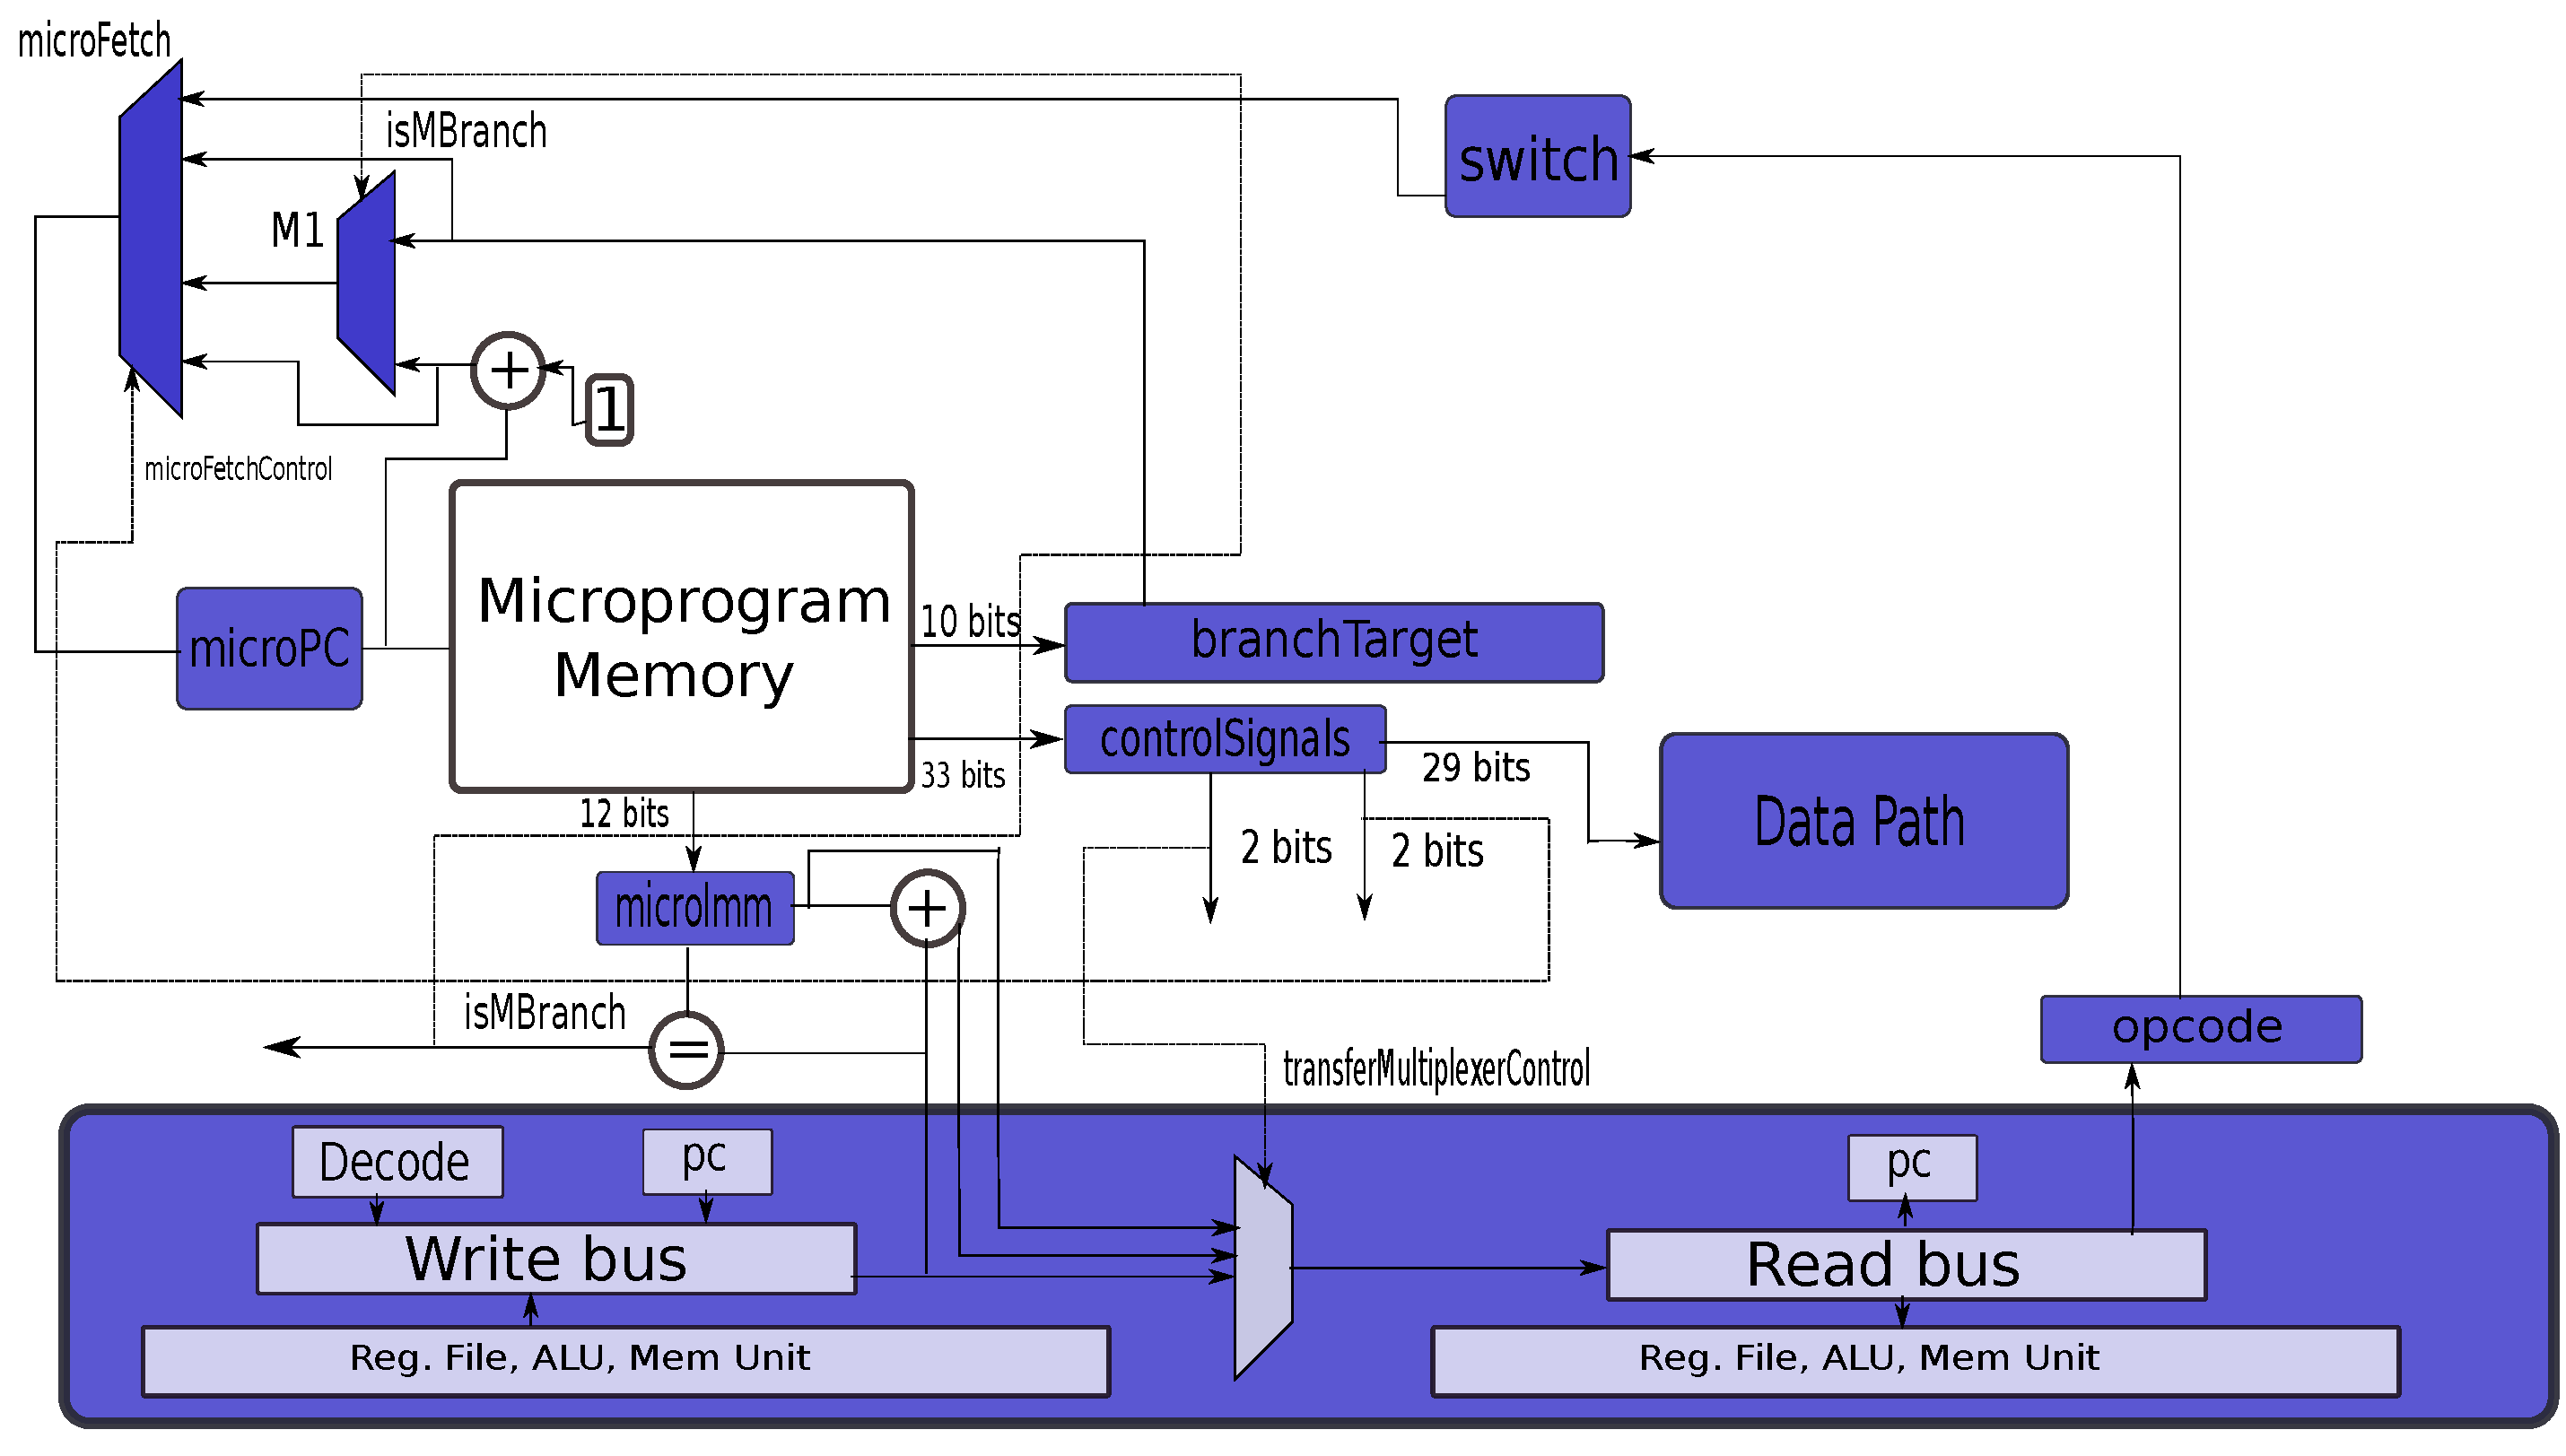
\includegraphics[width=12cm,height=14cm,keepaspectratio]{horizontalMP.pdf}
\end{figure}
\Exercise Compare the tradeoffs between horizontal and vertical microprogramming.
\Answer The tradeoffs between horizontal and vertical microprogramming are:\newline
1. Horizontal microprogramming requires more storage since it requires 65 bits for every instruction, when compared to that of 45 bits in vertical microprogramming. \newline
2. Horizontal microprogramming eliminates the need for dedicated signal generation logic in the $\mu$control unit.\newline
3. To program a horizontally microprogrammed processor, it is necessary to expose the control signals to the programmer and microassembler.This makes the microassembler specific to the processor. However, in case of vertical microprogramming, as long as the internal register set remains the same, we do not need different microassemblers.\newline
\end{ExerciseList}

\section*{Design Problems}

\begin{ExerciseList}
\Exercise
Implement the hardwired \simplerisc processor using Logisim, which is an educational tool for designing
and simulating digital circuits. It is freely available at \url{http://ozark.hendrix.edu/~burch/logisim}. 
Try to support all the instructions, and the modifiers.

\Exercise Now, try to implement a horizontally microprogrammed processor using Logisim. This project has
two parts.
\begin{enumerate}[a)]
\item Write a microassembler that can translate microassembly instructions to machine instructions. Use
this microassembler to generate the microcode for all the instructions in the \simplerisc ISA.
\item Create a data path and control path in Logisim for a horizontally microprogrammed processor.
This processor should be able to directly execute the code generated by the microassembler.
\item Run regular \simplerisc programs on this processor. 
\item Implement custom \simplerisc instructions such as $multiply-add$ (a $\leftarrow$ b*c + d), or instructions
to find the square of a number on this processor.
\end{enumerate}

\Exercise 
Implement the basic hardwired processor in a high level description language such as VHDL. You can use the
freely available open source tool, GNU HDL (\url{http://gna.org/projects/ghdl/}), to implement, and simulate
your circuit.

\end{ExerciseList}





































